% !TeX program = xelatex
\documentclass[UTF8,12pt,a4paper]{ctexart}

\usepackage{amsmath,amssymb,mathtools,bm}
\usepackage{graphicx}
\usepackage{geometry}
\usepackage{booktabs,tabularx,array,longtable,makecell,threeparttable}
\usepackage{subcaption}
\usepackage{float}
\usepackage[section]{placeins}
\usepackage{xcolor}
\usepackage{hyperref}
\usepackage{enumitem}
\usepackage{fancyhdr}
\usepackage{caption}
\usepackage{listings}
\usepackage{siunitx}
\usepackage{microtype}
\usepackage{url}

\geometry{left=2.35cm,right=2.35cm,top=2.35cm,bottom=2.45cm,headheight=15pt}
\setlength{\parindent}{2em}
\setlength{\parskip}{0.18em}
\setlength{\emergencystretch}{2em}
\renewcommand{\arraystretch}{1.16}
\setlist{nosep,leftmargin=2.2em}
\setcounter{tocdepth}{2}
\setcounter{secnumdepth}{3}

\definecolor{deepblue}{RGB}{28,68,116}
\definecolor{darkgreen}{RGB}{24,105,68}
\definecolor{darkred}{RGB}{160,45,45}
\definecolor{softgray}{RGB}{246,247,249}

\hypersetup{
  colorlinks=true,
  linkcolor=deepblue,
  urlcolor=deepblue,
  citecolor=deepblue,
  pdfauthor={冯海燕；陈奕帆},
  pdftitle={轮腿机器人姿态与运动控制对比研究}
}
\urlstyle{tt}

\pagestyle{fancy}
\fancyhf{}
\fancyhead[L]{轮腿机器人姿态与运动控制对比研究}
\fancyhead[R]{控制部分大作业二}
\fancyfoot[C]{\thepage}

\ctexset{
  section={format=\Large\bfseries\color{deepblue},beforeskip=1.1em,afterskip=0.7em},
  subsection={format=\large\bfseries,beforeskip=0.9em,afterskip=0.45em}
}
\captionsetup{font=small,labelfont=bf,skip=6pt}
\captionsetup[subfigure]{font=footnotesize,skip=3pt}
\sisetup{detect-all,per-mode=symbol}
\setlength{\textfloatsep}{0.75em plus 0.2em minus 0.2em}
\setlength{\floatsep}{0.65em plus 0.2em minus 0.2em}
\setlength{\intextsep}{0.75em plus 0.2em minus 0.2em}

\graphicspath{{outputs/compare_five_full_wbc/figures/}}
\newcommand{\code}[1]{\texttt{\detokenize{#1}}}
\newcommand{\good}{\textcolor{darkgreen}{未终止}}
\newcommand{\bad}{\textcolor{darkred}{终止}}
\newcommand{\comparisonfigwidth}{0.86\linewidth}
\newcolumntype{Y}{>{\raggedright\arraybackslash}X}
\newcolumntype{C}[1]{>{\centering\arraybackslash}p{#1}}

\lstdefinestyle{cmd}{
  basicstyle=\ttfamily\small,
  backgroundcolor=\color{softgray},
  frame=single,
  rulecolor=\color{black!20},
  breaklines=true,
  columns=fullflexible,
  keepspaces=true,
  showstringspaces=false,
  xleftmargin=0.5em,
  xrightmargin=0.5em
}

\begin{document}

\begin{titlepage}
  \centering
  \vspace*{2.0cm}
  {\zihao{2}\bfseries 控制部分大作业二\par}
  \vspace{1.0cm}
  {\zihao{-1}\bfseries 轮腿机器人姿态与运动控制对比研究\par}
  \vspace{0.8cm}
  {\zihao{3} 基于局部线性化 LQR、降阶 WBC/QP 与 PPO 的建模、实现及鲁棒性分析\par}
  \vfill
  \begin{tabular}{rl}
    学生：& 冯海燕、陈奕帆\\[0.4em]
    日期：& 2026 年 6 月
  \end{tabular}
  \vfill
  {\large 课程控制大作业报告\par}
\end{titlepage}

\pagenumbering{Roman}

\section*{摘要}
\addcontentsline{toc}{section}{摘要}
本文研究竖直平面内轮腿机器人的速度跟踪与姿态稳定问题。题目给定躯干质量为
\SI{50}{kg}，大腿和小腿长度均为 \SI{0.5}{m}，轮半径为 \SI{0.1}{m}，可控制轮毂、
膝关节和髋关节三路力矩；机器人需在 \SIrange{0}{5}{m/s} 的速度范围内抵抗不平整地形和
不超过 \SI{100}{N} 的水平质心扰动力。

为比较不同控制思想，本文在同一套二维降阶仿真模型上实现五种控制器：局部线性化
LQR、带显式动力学与约束的降阶 WBC/QP、基于 PD 稳定器的残差 PPO、仅保留模型前馈项的
残差 PPO 消融方案，以及直接输出三路力矩的 PPO。实验包含八个固定场景，每种实现各运行
一次，共得到 40 条确定性轨迹。评价指标包括安全终止状态、高度与姿态误差、速度误差、
力矩饱和比例以及平顺性和控制量代理指标。

统一评估结果显示：五种实现均未触发报告设定的安全终止阈值。降阶 WBC/QP 的八场景平均高度 RMSE 为
\SI{3.8e-4}{m}，平均姿态 RMSE 为 \SI{0.0095}{\degree}，在平台稳定性指标上最优；
直接力矩 PPO 的平均速度 RMSE 最低，为 \SI{0.082}{m/s}，但在 \SI{5}{m/s}、
\SI{100}{N} 与正弦地形叠加的边界场景中，姿态 RMSE 增至 \SI{4.06}{\degree}。
前馈残差消融方案虽然未触发安全阈值，但平均速度 RMSE 达到 \SI{2.888}{m/s}，说明安全判据、
速度性能与姿态性能必须分开评价。

此外，因为 WBC/QP 与前向仿真共享同一降阶模型和精确地形信息，仿真未加入参数失配、
传感器噪声、时延和复杂离地碰撞。本文据此给出控制器适用范围、实验有效性边界和后续改进方向。

\noindent\textbf{关键词：}轮腿机器人；LQR；全身控制；二次规划；PPO；鲁棒性分析

\clearpage
\tableofcontents
\clearpage
\pagenumbering{arabic}

\section{题目要求与研究范围}

\subsection{题目要求}
研究对象为竖直平面内运动的轮腿机器人，如图~\ref{fig:robot} 所示。机器人具有三路可控输入：
轮毂力矩 $\tau_{\rm wheel}$、膝关节力矩 $\tau_{\rm knee}$ 和髋关节力矩 $\tau_{\rm hip}$。
题目给定躯干质量、大腿长度、小腿长度和轮半径，并要求机器人在 \SIrange{0}{5}{m/s} 速度范围内
跟踪水平速度指令，同时承受不平整地形和作用于躯干质心处、幅值不超过 \SI{100}{N} 的水平扰动力。

本文将题目目标写成三个受控量：水平速度 $v_x$ 跟踪指令 $v_{\rm cmd}$，躯干俯仰角 $\theta$
跟踪零姿态，髋部绝对高度 $y$ 跟踪参考高度 $y_{\rm ref}$。三路力矩统一经过限幅后进入同一个
二维前向仿真模型，由同一组评价指标统计高度、姿态、速度和控制量表现。

\begin{figure}[htbp]
  \centering
  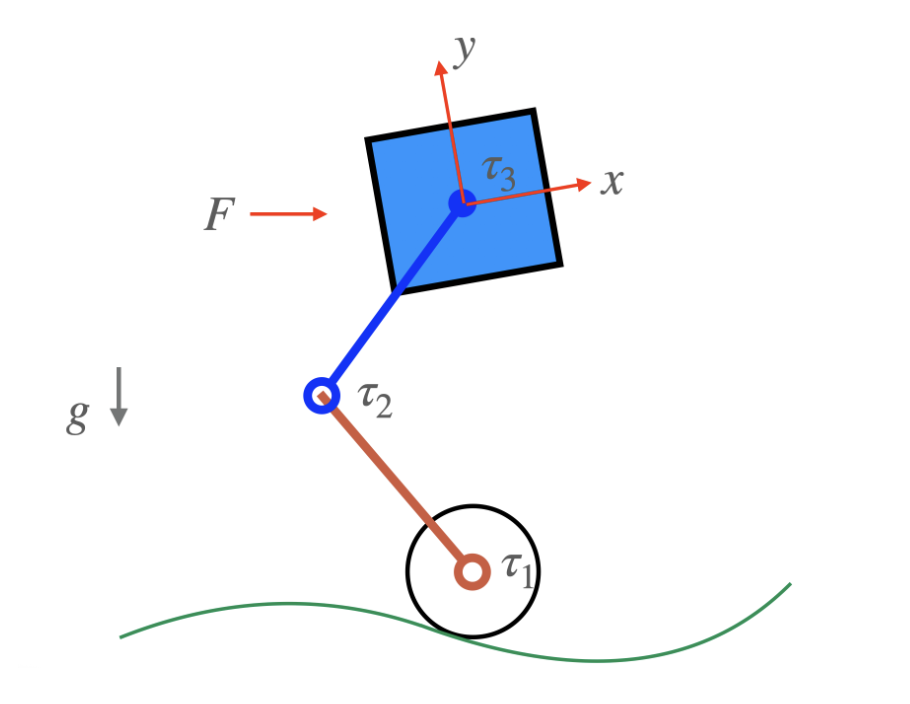
\includegraphics[width=0.74\linewidth]{robot.png}
  \caption{题目给出的轮腿机器人示意图。本文把水平外力作为通过躯干质心的平动力处理。}
  \label{fig:robot}
\end{figure}

\subsection{研究路线与控制器分组}
轮腿机器人兼具轮式移动效率和腿式地形适应能力，相关系统常将任务空间控制、全身约束优化和学习控制结合起来
实现稳定运动\cite{Bjelonic2019KeepRollin}。本文在同一仿真平台上实现五种控制器：局部线性化 LQR、
降阶 WBC/QP、PD 残差 PPO、前馈残差 PPO 和直接力矩 PPO。其中 LQR 作为模型反馈基线，WBC/QP 作为
约束优化控制器，三种 PPO 用于比较不同学习控制结构。

统一仿真流程为：固定场景给出地形、速度指令和水平外力；控制器根据其观测信息输出
$[\tau_{\rm wheel},\tau_{\rm knee},\tau_{\rm hip}]^{\mathsf T}$；动力学模块对力矩限幅后计算接触力和
状态导数；四阶 Runge--Kutta 积分推进状态；日志模块保存轨迹；评价模块输出指标。各控制器共享被控对象、
仿真步长、执行器限幅、安全判据和测试场景。实现层面的观测信息为：LQR 使用状态和速度指令，WBC/QP
使用当前地形并在预测约束中查询短时前方地形，PPO 使用由状态和局部地形高度、坡度组成的观测向量。

\subsection{参数设定}
表~\ref{tab:params} 汇总代码中使用的主要机器人参数、仿真参数和控制器动作尺度。

\begin{table}[htbp]
\centering
\caption{机器人与仿真参数}
\label{tab:params}
\small
\begin{threeparttable}
\begin{tabularx}{\linewidth}{lC{2.4cm}C{2.8cm}Y}
\toprule
参数 & 符号 & 数值 & 来源或作用 \\
\midrule
躯干质量 & $m$ & \SI{50}{kg} & 题目给定 \\
大腿长度 & $L_1$ & \SI{0.5}{m} & 题目给定 \\
小腿长度 & $L_2$ & \SI{0.5}{m} & 题目给定 \\
轮半径 & $r$ & \SI{0.1}{m} & 题目给定 \\
重力加速度 & $g$ & \SI{9.81}{m/s^2} & 常规取值 \\
躯干等效转动惯量 & $I$ & \SI{5.0}{kg.m^2} & 降阶模型设定 \\
轮地摩擦系数 & $\mu$ & $0.8$ & 接触模型设定 \\
期望髋部高度 & $y_{\rm ref}$ & \SI{0.82}{m} & 统一测试参考值 \\
腿部平衡长度 & $l_0$ & \SI{0.72}{m} & 被动支撑模型设定 \\
腿部等效刚度 & $k_l$ & \SI{900}{N/m} & 被动支撑模型设定 \\
腿部等效阻尼 & $c_l$ & \SI{55}{N.s/m} & 被动支撑模型设定 \\
水平阻尼系数 & $c_x$ & $10.0$ & 水平速度阻尼 \\
竖直阻尼系数 & $c_y$ & $35.0$ & 竖直速度阻尼 \\
姿态等效刚度 & $k_\theta$ & $18.0$ & 躯干俯仰回复项 \\
姿态等效阻尼 & $c_\theta$ & $2.8$ & 躯干角速度阻尼 \\
腿部等效力臂 & $d$ & \SI{0.25}{m} & 膝髋力矩到竖直支撑力的映射 \\
俯仰耦合比例 & $\gamma$ & $0.25$ & 切向接触力到躯干俯仰的等效传递比例 \\
仿真步长 & $\Delta t$ & \SI{0.01}{s} & \SI{100}{Hz} 控制周期 \\
单次时长 & $T$ & \SI{8}{s} & 固定场景时长 \\
高度失败阈值 & $h_{\rm fail}$ & \SI{0.15}{m} & 髋部高度安全判据 \\
最小腿长阈值 & $l_{\rm safety}$ & \SI{0.18}{m} & 腿部塌缩安全判据 \\
力矩上限 & $\bm\tau_{\max}$ & $[30,160,120]^{\mathsf T}$ \si{N.m} & 轮、膝、髋三路人为限幅 \\
残差动作尺度 & $\bm s_{\rm res}$ & $[5,25,25]^{\mathsf T}$ \si{N.m} & PD 残差 PPO 使用 \\
\bottomrule
\end{tabularx}
\begin{tablenotes}[flushleft]\footnotesize
\item 注：质量、腿长和轮半径来自题目，其余参数由仿真模型和控制器实现统一给定。
\end{tablenotes}
\end{threeparttable}
\end{table}

\section{二维降阶仿真模型}

\subsection{状态、输入与地形}
仿真状态取髋部平动、躯干俯仰及其速度：
\begin{align}
\bm x&=[x,\ y,\ \theta,\ v_x,\ v_y,\ \omega]^{\mathsf T},\\
\bm\tau&=[\tau_{\rm wheel},\ \tau_{\rm knee},\ \tau_{\rm hip}]^{\mathsf T}.
\end{align}
其中 $x,y$ 为髋部位置，$\theta$ 为躯干俯仰角，$v_x,v_y$ 为髋部速度，$\omega$ 为俯仰角速度。
地形对象统一提供高度 $h(x)$、坡度 $h'(x)$ 和曲率 $h''(x)$。平地直接给出零高度和零坡度；正弦地形采用
解析导数；多频地形把多个正弦分量叠加后按最大高度缩放；随机地形先采样高斯高度，再用卷积平滑和三次样条
生成连续高度、坡度和曲率。

\subsection{轮腿几何与可达性}
轮心高度由地形高度和轮半径给出：
\begin{equation}
y_{\rm wheel}=h(x)+r.
\end{equation}
代码把两段腿的支撑效果写成竖直伸缩腿，腿长和腿长变化率为
\begin{align}
l&=y-y_{\rm wheel}=y-h(x)-r,\\
\dot l&=v_y-h'(x)v_x .
\end{align}
逆运动学函数用两连杆长度检查该腿长是否可达。设两段长度为 $L_1,L_2$，内部膝角满足
\begin{equation}
\cos\beta_{\rm int}=\frac{L_1^2+L_2^2-l_c^2}{2L_1L_2},
\end{equation}
其中 $l_c$ 是裁剪到 $(0,L_1+L_2)$ 内的腿长。代码定义膝屈曲角
\begin{equation}
\beta_{\rm knee}=\pi-\beta_{\rm int},
\end{equation}
并取
\begin{equation}
q_{\rm hip}=\frac12\beta_{\rm knee}.
\end{equation}
这两个角度用于构造腿部几何量和 PPO 观测，安全判定使用原始腿长 $l$ 的可达性。

\subsection{力矩限幅与接触力}
所有控制器输出先经过统一执行器限幅：
\begin{equation}
\bm\tau=\operatorname{clip}(\bm\tau_{\rm cmd},-\bm\tau_{\max},\bm\tau_{\max}).
\end{equation}
膝关节和髋关节力矩通过等效力臂 $d=\SI{0.25}{m}$ 形成主动腿部支撑力：
\begin{align}
F_{\rm leg,act}&=\frac{\tau_{\rm knee}+0.6\tau_{\rm hip}}{d},\\
F_{\rm leg,pass}&=k_l(l_0-l)-c_l\dot l,\\
F_{\rm leg}&=F_{\rm leg,act}+F_{\rm leg,pass}.
\end{align}
轮毂力矩形成期望切向驱动力
\begin{equation}
F_{\rm drive,cmd}=\frac{\tau_{\rm wheel}}{r}.
\end{equation}
接触法向力和切向力按
\begin{align}
F_n&=\max(F_{\rm leg},0),\\
F_t&=\operatorname{clip}\!\left(F_{\rm drive,cmd},-\mu\max(F_n,1),\mu\max(F_n,1)\right)
\end{align}
计算。这里的切向力限幅对应二维库仑摩擦约束，$\max(F_n,1)$ 用于法向力很小时的数值保护。

\subsection{前向动力学与积分}
动力学模块把轮地切向力、腿部支撑力、阻尼、坡度阻力和外力合成为三个加速度：
\begin{align}
\ddot x&=\frac{F_t+F_{\rm ext}-c_xv_x-mgh'(x)}{m},\\
\ddot y&=\frac{F_{\rm leg}-mg-c_yv_y}{m},\\
\ddot\theta&=\frac{\tau_{\rm hip}+0.15\tau_{\rm knee}+d_tF_t-k_\theta\theta-c_\theta\omega}{I},
\end{align}
其中轮地切向力到躯干俯仰的等效力臂为
\begin{equation}
d_t=\gamma\max(y-h(x),0.1).
\end{equation}
因此状态导数为
\begin{equation}
\dot{\bm x}=[v_x,\ v_y,\ \omega,\ \ddot x,\ \ddot y,\ \ddot\theta]^{\mathsf T}.
\end{equation}
单步推进使用四阶 Runge--Kutta：
\begin{align}
\bm k_1&=f(\bm x_k,\bm\tau_k),\\
\bm k_2&=f(\bm x_k+\tfrac12\Delta t\bm k_1,\bm\tau_k),\\
\bm k_3&=f(\bm x_k+\tfrac12\Delta t\bm k_2,\bm\tau_k),\\
\bm k_4&=f(\bm x_k+\Delta t\bm k_3,\bm\tau_k),\\
\bm x_{k+1}&=\bm x_k+\frac{\Delta t}{6}(\bm k_1+2\bm k_2+2\bm k_3+\bm k_4).
\end{align}
其中 $f(\bm x,\bm\tau)$ 表示由前向动力学计算出的状态导数函数，$\bm k_1$ 至 $\bm k_4$
是 Runge--Kutta 方法在一个步长内的四次斜率估计。
日志中保存推进后状态对应的加速度、接触力、饱和状态和控制器诊断量。

\subsection{安全终止判据}
每个积分步后检查安全状态：
\begin{enumerate}
  \item $|\theta|>\SI{30}{\degree}$，记为 \code{theta_fail}；
  \item $|y-y_{\rm ref}|>\SI{0.15}{m}$，记为 \code{height_fail}；
  \item 腿长超出 $r\le l\le L_1+L_2$，记为 \code{leg_infeasible}；
  \item $l<\SI{0.18}{m}$，记为 \code{leg_collapsed}。
\end{enumerate}
若触发任一条件，仿真记录失败原因；默认评估在首次失败后停止。

\section{评价指标}

\subsection{轨迹日志}
每次仿真保存从 $t=0$ 到终止时刻的采样序列。日志包含状态、速度指令、参考高度、真实外力、地形高度与坡度、
轮心高度、腿长、三路力矩、法向/切向接触力、三向加速度、饱和标志、失败标志以及 WBC/QP 诊断量。若场景完整运行
\SI{8}{s}，在 $\Delta t=\SI{0.01}{s}$ 下共有 801 个采样点。

\subsection{核心指标}
设日志采样点数为 $N$，评价模块首先根据失败原因定义
\begin{equation}
S=\begin{cases}
1,&\text{未记录失败原因},\\
0,&\text{记录了失败原因}.
\end{cases}
\end{equation}
高度、姿态和速度误差指标为
\begin{align}
\mathrm{RMSE}_h&=\sqrt{\frac{1}{N}\sum_{k=1}^{N}(y_k-y_{{\rm ref},k})^2},\\
e_{h,\max}&=\max_k|y_k-y_{{\rm ref},k}|,\\
\mathrm{RMSE}_\theta&=\sqrt{\frac{1}{N}\sum_{k=1}^{N}\theta_k^2},\\
\theta_{\max}&=\max_k|\theta_k|,\\
\mathrm{RMSE}_v&=\sqrt{\frac{1}{N}\sum_{k=1}^{N}(v_{x,k}-v_{{\rm cmd},k})^2}.
\end{align}
表格中的姿态 RMSE 和最大姿态角统一换算为角度。力矩饱和比例按三路力矩的全部采样元素统计：
\begin{equation}
\rho_{\rm sat}=
\frac{1}{3N}\sum_{k=1}^{N}\sum_{i=1}^{3}
\mathbf 1\!\left(\frac{|\tau_{i,k}|}{\tau_{i,\max}}\ge0.98\right).
\end{equation}

评价模块还计算水平加速度变化和平动/转动动态响应组成的平顺性代理量：
\begin{equation}
J_s=\int\left(\dot a_x^2+0.1\alpha^2\right)\,\mathrm dt,
\end{equation}
其中 $\alpha=\ddot\theta$，$\dot a_x$ 由离散梯度 \code{np.gradient} 计算。力矩平方积分为
\begin{equation}
E_\tau=\int\left(\tau_{\rm wheel}^2+\tau_{\rm knee}^2+\tau_{\rm hip}^2\right)\,\mathrm dt.
\end{equation}
两个积分均由梯形积分实现。WBC/QP 轨迹额外统计 QP 成功比例、OSQP 成功比例、回退比例、平均迭代次数、
平均/最大求解耗时、约束残差、摩擦利用率和安全松弛量。



\section{局部线性化 LQR}

\subsection{方法特点}
LQR 是经典线性二次型最优控制方法\cite{Kalman1960OptimalControl,AndersonMoore1990OptimalControl}。
它先把非线性系统在工作点附近写成线性模型
\begin{equation}
\Delta\dot{\bm x}=A\Delta\bm x+B\Delta\bm\tau,
\end{equation}
再最小化二次型性能指标
\begin{equation}
J=\int_0^\infty
\left(\Delta\bm x^{\mathsf T}Q\Delta\bm x+\Delta\bm\tau^{\mathsf T}R\Delta\bm\tau\right)\mathrm dt .
\end{equation}
该方法控制律为线性状态反馈，结构清晰、在线计算量小，适合用作局部稳定控制基线；其控制性能由线性化工作点和
权重矩阵共同决定。

\subsection{方法实现}
LQR 控制器在平地、无外力条件下按当前速度指令 $v_{\rm cmd}$ 构造名义状态
\begin{equation}
\bm x_0=[0,\ y_{\rm ref},\ 0,\ v_{\rm cmd},\ 0,\ 0]^{\mathsf T}.
\end{equation}
代码中的平衡力矩由 \code{equilibrium_torque} 给出。轮毂力矩抵消水平阻尼：
\begin{equation}
\tau_{{\rm wheel},0}=c_xv_{\rm cmd}r,
\end{equation}
对应名义切向力 $F_{t,0}=c_xv_{\rm cmd}$。膝、髋力矩由主动支撑力和俯仰力矩两个方程确定：
\begin{equation}
\begin{bmatrix}
1 & 0.6\\
0.15 & 1
\end{bmatrix}
\begin{bmatrix}
\tau_{{\rm knee},0}\\
\tau_{{\rm hip},0}
\end{bmatrix}
=
\begin{bmatrix}
dmg\\
-d_{t,0}F_{t,0}
\end{bmatrix},
\end{equation}
其中
\begin{equation}
d_{t,0}=\gamma(l_0+r).
\end{equation}

在该工作点附近，代码用中心差分计算 $A$ 和 $B$。差分步长为 $\epsilon=10^{-5}$：
\begin{align}
A_{:,i}&=\frac{f(\bm x_0+\epsilon\bm e_i,\bm\tau_0)-f(\bm x_0-\epsilon\bm e_i,\bm\tau_0)}{2\epsilon},\\
B_{:,j}&=\frac{f(\bm x_0,\bm\tau_0+\epsilon\bm e_j)-f(\bm x_0,\bm\tau_0-\epsilon\bm e_j)}{2\epsilon}.
\end{align}
其中 $f(\bm x,\bm\tau)$ 为状态导数函数，$\bm e_i$ 和 $\bm e_j$ 分别为状态空间和输入空间中的单位基向量，
$\epsilon$ 为中心差分扰动步长。
状态权重和输入权重为
\begin{align}
Q&=\operatorname{diag}(0,\ 600,\ 1800,\ 30,\ 120,\ 280),\\
R&=\operatorname{diag}(0.03,\ 0.06,\ 0.05).
\end{align}
连续代数 Riccati 方程
\begin{equation}
A^{\mathsf T}P+PA-PBR^{-1}B^{\mathsf T}P+Q=0
\end{equation}
给出反馈矩阵
\begin{equation}
K=R^{-1}B^{\mathsf T}P.
\end{equation}
其中 $P$ 为 Riccati 方程的对称正定解，$K$ 为用于在线反馈的状态增益矩阵。

在线控制时，参考状态取为
\begin{equation}
\bm x_{\rm ref}=[x,\ y_{\rm ref},\ 0,\ v_{\rm cmd},\ 0,\ 0]^{\mathsf T},
\end{equation}
因此反馈误差为
\begin{equation}
\bm x-\bm x_{\rm ref}=[0,\ y-y_{\rm ref},\ \theta,\ v_x-v_{\rm cmd},\ v_y,\ \omega]^{\mathsf T}.
\end{equation}
控制律为
\begin{equation}
\bm\tau=\operatorname{clip}\!\left(\bm\tau_0-K(\bm x-\bm x_{\rm ref}),
-\bm\tau_{\max},\bm\tau_{\max}\right).
\end{equation}
增益按照四舍五入到两位小数的速度指令缓存，避免重复求解 Riccati 方程。

\section{降阶 WBC/QP 控制器}

\subsection{方法特点}
全身控制和操作空间控制把机器人任务、接触力、执行器力矩和物理约束放入统一控制框架
\cite{Khatib1987OperationalSpace}。QP 形式的优点是任务目标和约束可以直接写入优化问题；其在线计算由
二次规划求解器完成，适合表达摩擦、法向力、力矩边界和预测安全边界。本文模型已经把腿部几何降阶为竖直腿长，
因此控制器实现为降阶任务空间 WBC/QP。

\subsection{决策变量与任务目标}
每个控制周期的决策变量为
\begin{equation}
\bm z=[a_x,a_y,\alpha,F_t,F_n,\tau_{\rm wheel},\tau_{\rm knee},\tau_{\rm hip},
 s_{l,-},s_{l,+},s_{y,-},s_{y,+}]^{\mathsf T}.
\end{equation}
前三项为任务空间加速度，$F_t,F_n$ 为切向和法向接触力，后三个力矩为控制输出，四个松弛变量用于预测腿长和
预测高度边界。

期望任务加速度由速度、高度和姿态误差给出：
\begin{align}
e_{v,I}&\leftarrow\operatorname{clip}\!\left(e_{v,I}+\Delta t(v_{\rm cmd}-v_x),-2,2\right),\\
a_{x,\rm des}&=5(v_{\rm cmd}-v_x)+2e_{v,I},\\
a_{y,\rm des}&=115(y_{\rm ref}-y)-24v_y,\\
\alpha_{\rm des}&=-125\theta-24\omega.
\end{align}
其中 $e_{v,I}$ 为速度误差积分状态，控制器重置时置零。

\subsection{动力学等式约束}
WBC/QP 使用与前向动力学一致的仿射模型。固定当前状态、地形和控制器可用外力估计 $\hat F_{\rm ext}$ 后，
平动方程给出
\begin{align}
ma_x-F_t&=\hat F_{\rm ext}-c_xv_x-mgh'(x),\\
ma_y-F_n&=-mg-c_yv_y.
\end{align}
俯仰动力学写为
\begin{equation}
I\alpha-d_tF_t-0.15\tau_{\rm knee}-\tau_{\rm hip}
=-k_\theta\theta-c_\theta\omega,
\end{equation}
其中 $d_t=\gamma\max(y-h(x),0.1)$。轮毂力矩与切向力、膝髋力矩与法向力之间的执行器映射为
\begin{align}
\tau_{\rm wheel}-rF_t&=0,\\
\tau_{\rm knee}+0.6\tau_{\rm hip}-dF_n&=-dF_{\rm leg,pass},
\end{align}
其中
\begin{equation}
F_{\rm leg,pass}=k_l(l_0-l)-c_l\dot l.
\end{equation}
其中 $\hat F_{\rm ext}$ 表示控制器可用的水平外力估计量。正式评估默认不启用外力测量开关，
因此控制器使用 $\hat F_{\rm ext}=0$；真实外力仍进入前向动力学。

\subsection{不等式约束与预测边界}
硬约束包括法向预载、摩擦锥、力矩边界和松弛变量非负：
\begin{align}
F_n&\ge0.35mg,\\
F_t-\mu F_n&\le0,\\
-F_t-\mu F_n&\le0,\\
-\bm\tau_{\max}&\le\bm\tau\le\bm\tau_{\max},\\
s_{l,-},s_{l,+},s_{y,-},s_{y,+}&\ge0.
\end{align}

预测时域为 $T_p=\SI{0.30}{s}$。代码先以当前速度预瞄位置
\begin{equation}
x_p=x+T_pv_x
\end{equation}
查询前方地形，并用待优化加速度修正未来高度和腿长：
\begin{align}
y_p&=y+T_pv_y+\frac12T_p^2a_y,\\
l_p&=y+T_pv_y-h(x_p)-r
+\frac12T_p^2a_y-\frac12T_p^2h'(x_p)a_x.
\end{align}
边界取
\begin{align}
l_{\min}&=l_{\rm safety}+0.02,\qquad
l_{\max}=L_1+L_2-0.02,\\
y_{\min}&=y_{\rm ref}-h_{\rm fail}+0.01,\qquad
y_{\max}=y_{\rm ref}+h_{\rm fail}-0.01.
\end{align}
预测约束写成
\begin{align}
l_p+s_{l,-}&\ge l_{\min},&
l_p-s_{l,+}&\le l_{\max},\\
y_p+s_{y,-}&\ge y_{\min},&
y_p-s_{y,+}&\le y_{\max}.
\end{align}
其中 $l_{\rm safety}$ 为安全判据中的最小腿长阈值，$h_{\rm fail}$ 为高度偏差失败阈值；
$s_{l,-},s_{l,+}$ 分别表示腿长下界和上界松弛量，$s_{y,-},s_{y,+}$ 分别表示高度下界和上界松弛量。

\subsection{二次规划目标与求解}
目标函数采用加权二次型：
\begin{align}
\min_{\bm z}\quad
&\frac12\|\bm a-\bm a_{\rm des}\|_{W_a}^2
+\frac{w_\tau}{2}\left\|\frac{\bm\tau}{\bm\tau_{\max}}\right\|_2^2
+\frac{w_{\Delta\tau}}{2}\left\|\frac{\bm\tau-\bm\tau_{\rm last}}{\bm\tau_{\max}}\right\|_2^2\nonumber\\
&+\frac{w_f}{2}\left[
\left(\frac{F_t}{\tau_{{\rm wheel},\max}/r}\right)^2
+\left(\frac{F_n-mg}{mg}\right)^2
\right]
+\frac{w_l}{2}(s_{l,-}^2+s_{l,+}^2)
+\frac{w_y}{2}(s_{y,-}^2+s_{y,+}^2).
\end{align}
代码中的权重为
\begin{align}
W_a&=\operatorname{diag}(8,\ 180,\ 120),\\
w_\tau&=0.03,\quad
w_{\Delta\tau}=0.12,\quad
w_f=0.002,\quad
w_l=4\times10^5,\quad
w_y=6\times10^5.
\end{align}
问题被装配为 OSQP 标准形式
\begin{equation}
\min_{\bm z}\frac12\bm z^{\mathsf T}P\bm z+\bm q^{\mathsf T}\bm z
\quad\mathrm{s.t.}\quad
\bm l\le A\bm z\le\bm u,
\end{equation}
其中 $P$ 和 $\bm q$ 分别为 QP 目标函数的 Hessian 矩阵和线性项，$A$ 为等式、不等式和变量边界拼接后的
约束矩阵，$\bm l,\bm u$ 为对应的下界和上界。
并由 OSQP 求解\cite{Stellato2020OSQP}。若候选解为非有限值、求解状态未成功，或等式/不等式残差超过阈值，
控制器使用由稳定基线力矩构造的初始可行解。最终输出为 $\bm z$ 中三路力矩分量的限幅结果。

\section{PPO 强化学习控制}

\subsection{方法特点}
PPO 是基于策略梯度的强化学习算法，通过限制新旧策略概率比的变化幅度提高训练稳定性
\cite{Schulman2017PPO}。在控制问题中，PPO 直接学习从观测 $\bm o$ 到动作 $\bm u$ 的非线性映射，
适合表示难以手工线性化的反馈律；训练完成后，在线控制只需一次神经网络前向推理。本文通过 Gymnasium 环境接口
和 Stable-Baselines3 完成训练与模型加载\cite{Towers2024Gymnasium,Raffin2021SB3}。

\subsection{环境观测与奖励}
策略动作是三维归一化向量
\begin{equation}
\bm u=[u_1,u_2,u_3]^{\mathsf T}\in[-1,1]^3.
\end{equation}
观测向量由状态误差、腿长、局部地形和速度指令构成：
\begin{equation}
\bm o=[y-y_{\rm ref},\theta,v_x-v_{\rm cmd},v_y,\omega,l,h(x),h'(x),v_{\rm cmd}]^{\mathsf T}.
\end{equation}
训练环境重置时，初始状态在 $[0,y_{\rm ref},0,0,0,0]^{\mathsf T}$ 附近随机扰动：
\begin{align}
y&\leftarrow y_{\rm ref}+\mathcal N(0,0.01^2),&
\theta&\leftarrow \mathcal N(0,\operatorname{deg}(0.8)^2),\\
v_x&\leftarrow \mathcal N(0,0.04^2),&
v_y&\leftarrow \mathcal N(0,0.02^2),&
\omega&\leftarrow \mathcal N(0,\operatorname{deg}(1.0)^2).
\end{align}
其中 $\mathcal N(\mu,\sigma^2)$ 表示均值为 $\mu$、方差为 $\sigma^2$ 的高斯分布；
$\operatorname{deg}(\cdot)$ 表示将角度值换算为弧度。

单步奖励由高度、姿态、速度、动作幅值、动态响应和终止状态组成：
\begin{align}
r={}&0.5
+3.5e^{-130(y-y_{\rm ref})^2}
+2.5e^{-45\theta^2}
+1.2e^{-0.7(v_x-v_{\rm cmd})^2}\nonumber\\
&-35(y-y_{\rm ref})^2
-3\theta^2
-c_u\|\bm u\|_2^2
-0.001\|[\ddot x,\ddot y,\ddot\theta]^{\mathsf T}\|_2^2
+r_{\rm mode}+r_{\rm sat}+r_{\rm fail}.
\end{align}
其中 $c_u$ 为动作二范数惩罚权重，$r_{\rm mode}$ 为不同动作模式附加的奖励项，
$r_{\rm sat}$ 为动作接近饱和时的惩罚项，$r_{\rm fail}$ 为触发安全终止时的惩罚项。残差类动作
$c_u=0.03$，直接力矩动作 $c_u=0.008$。直接力矩模式额外加入
\begin{equation}
r_{\rm mode}=-0.004\sum_{i=1}^{3}\left(\frac{\tau_i}{\tau_{i,\max}}\right)^2,
\end{equation}
其余模式 $r_{\rm mode}=0$。若任一动作满足 $|u_i|>0.98$，则 $r_{\rm sat}=-0.5$，否则为零；
若触发安全终止，则 $r_{\rm fail}=-50$，否则为零。

\subsection{PD 残差 PPO}
PD 残差模式先由稳定基线控制器计算基础力矩，再叠加 PPO 输出的有限幅值残差。基础控制器的期望加速度为
\begin{align}
a_{x,\rm cmd}&=3(v_{\rm cmd}-v_x)-\frac{\hat F_{\rm ext}}{m},\\
a_{y,\rm cmd}&=70(y_{\rm ref}-y)-16v_y,\\
\alpha_{\rm cmd}&=-85\theta-18\omega.
\end{align}
轮毂力矩为
\begin{equation}
\tau_{\rm wheel}=r(c_xv_{\rm cmd}+ma_{x,\rm cmd}),
\end{equation}
腿部支撑力为
\begin{equation}
F_{\rm leg}=\max\{m(g+a_{y,\rm cmd}),0\}.
\end{equation}
俯仰任务所需关节力矩满足
\begin{equation}
\begin{bmatrix}
1 & 0.6\\
0.15 & 1
\end{bmatrix}
\begin{bmatrix}
\tau_{\rm knee}\\
\tau_{\rm hip}
\end{bmatrix}
=
\begin{bmatrix}
dF_{\rm leg}\\
I\alpha_{\rm cmd}+k_\theta\theta+c_\theta\omega-\gamma\max(y,0.1)\frac{\tau_{\rm wheel}}{r}
\end{bmatrix}.
\end{equation}
PPO 输出按残差尺度 $\bm s_{\rm res}=[5,25,25]^{\mathsf T}$ 叠加：
\begin{equation}
\bm\tau=\operatorname{clip}\!\left(\bm\tau_{\rm base}+\bm u\odot\bm s_{\rm res},
-\bm\tau_{\max},\bm\tau_{\max}\right).
\end{equation}

\subsection{前馈残差 PPO}
前馈残差模式使用地形模型计算名义前馈力矩，再由 PPO 输出残差。代码首先计算
\begin{align}
l_{\rm nom}&=y_{\rm ref}-h(x)-r,\\
\dot l_{\rm nom}&=-h'(x)v_{\rm cmd},\\
F_t^\star&=c_xv_{\rm cmd}+mgh'(x)-\hat F_{\rm ext},\\
F_n^\star&=mg.
\end{align}
被动支撑力为
\begin{equation}
F_{\rm pass}^\star=k_l(l_0-l_{\rm nom})-c_l\dot l_{\rm nom},
\end{equation}
主动支撑力为
\begin{equation}
F_{\rm act}^\star=F_n^\star-F_{\rm pass}^\star.
\end{equation}
名义轮毂力矩和膝髋力矩由
\begin{align}
\tau_{\rm wheel}^\star&=rF_t^\star,\\
\begin{bmatrix}
1 & 0.6\\
0.15 & 1
\end{bmatrix}
\begin{bmatrix}
\tau_{\rm knee}^\star\\
\tau_{\rm hip}^\star
\end{bmatrix}
&=
\begin{bmatrix}
dF_{\rm act}^\star\\
-\gamma\max(y_{\rm ref}-h(x),0.1)F_t^\star
\end{bmatrix}
\end{align}
得到。最终动作映射与残差模式相同：
\begin{equation}
\bm\tau=\operatorname{clip}\!\left(\bm\tau_{\rm ff}+\bm u\odot\bm s_{\rm res},
-\bm\tau_{\max},\bm\tau_{\max}\right).
\end{equation}

\subsection{直接力矩 PPO}
直接力矩 PPO 不叠加基础控制器，直接把三维动作映射为三路力矩：
\begin{align}
\tau_{\rm wheel}&=u_1\tau_{{\rm wheel},\max}=30u_1,\\
\tau_{\rm knee}&=\frac{u_2+1}{2}\tau_{{\rm knee},\max}=80(u_2+1),\\
\tau_{\rm hip}&=u_3\tau_{{\rm hip},\max}=120u_3.
\end{align}
膝关节通道映射到 $[0,160]$ \si{N.m}，轮毂和髋关节通道映射到对称区间。三路力矩随后仍经过统一限幅函数。

\subsection{训练配置}
训练脚本使用 Stable-Baselines3 的 PPO。新建模型时，残差类策略采用学习率 $2\times10^{-4}$、
熵系数 $0.003$；直接力矩策略采用学习率 $3\times10^{-4}$、熵系数 $0.008$。公共超参数为
\begin{equation}
n_{\rm steps}=1024,\quad
\text{batch size}=256,\quad
\gamma=0.99,\quad
\lambda_{\rm GAE}=0.95,\quad
\epsilon_{\rm clip}=0.2.
\end{equation}
其中 $\lambda_{\rm GAE}$ 为广义优势估计参数，$\epsilon_{\rm clip}$ 为 PPO 概率比裁剪范围。
固定场景评估时，控制器通过 \code{model.predict(obs, deterministic=True)} 调用训练好的策略。

\section{固定场景与数据来源}

\subsection{八个固定场景}

为覆盖题目中的速度范围、地形起伏和水平外力扰动，本文设计了八个固定测试场景，如下表：场景 A 至 D 分别考察瞬态外力、持续外力、规则地形、平滑随机地形和大幅不规则地形等单一因素；场景 E 用于复合压力测试；场景 F 和 G 分别检验 \SI{5}{m/s} 高速跟踪以及最高速度、最大外力、不平地形同时出现时的边界工况。

\begin{table}[htbp]
\centering
\caption{固定测试场景}
\label{tab:scenarios}
\small
\begin{tabularx}{\linewidth}{C{2.9cm}C{1.7cm}C{4.6cm}Y}
\toprule
场景 & 指令速度 & 水平外力 & 地形 \\
\midrule
A：瞬态强冲击 & \SI{2}{m/s} & $t=\SI{5}{s}$ 时施加 \SI{100}{N}，持续 \SI{0.1}{s} & 平地 \\
B：持续恒定推力 & \SI{3}{m/s} & 持续 \SI{80}{N} & 平地 \\
C1：规则正弦地形 & \SI{2}{m/s} & 无 & 振幅 \SI{0.05}{m}、波长 \SI{1.0}{m} \\
C2：平滑随机地形 & \SI{2}{m/s} & 无 & 振幅参数 \SI{0.04}{m}、固定随机种子 7 \\
D：大幅不规则地形 & \SI{2}{m/s} & 无 & 三频正弦叠加，最大绝对高度约 \SI{0.085}{m} \\
E：超规格组合压力 & \SI{3}{m/s} & 持续 \SI{60}{N}，$t=\SI{4}{s}$ 叠加 \SI{100}{N} 脉冲，峰值 \SI{160}{N} & 三频正弦叠加，最大绝对高度约 \SI{0.090}{m} \\
F：高速平地 & \SI{5}{m/s} & 无 & 平地 \\
G：边界组合 & \SI{5}{m/s} & 持续 \SI{100}{N} & 振幅 \SI{0.05}{m}、波长 \SI{1.0}{m} \\
\bottomrule
\end{tabularx}
\end{table}

表中速度为稳态目标值；当前代码通过 \code{smooth_speed} 在约 \SI{1}{s}
内从零平滑上升到目标速度，因此速度 RMSE 包含启动过程。

\subsection{数据批次与图表说明}
报告采用目录 \code{outputs/compare_five_full_wbc} 中的统一批次结果：五种实现、八个场景，共 40 条轨迹。
当前工作区保留了该批次的 \code{metrics.csv} 与 \code{figures/} 图像文件；若需要逐采样点日志或
WBC/QP 诊断原始数组，应重新运行评估脚本生成 \code{logs/} 目录。提交时还应保留运行命令、随机种子、
模型哈希和软件版本。

\section{总体结果与有效性分析}

\subsection{八场景汇总}
\begin{table}[htbp]
\centering
\caption{五种实现的八场景平均结果}
\label{tab:aggregate}
\small
\begin{threeparttable}
\begin{tabular}{lcccccc}
\toprule
控制器 & 未终止 & 高度 RMSE/m & 姿态 RMSE/$^\circ$ & 速度 RMSE/(m/s) & 饱和比例 \\
\midrule
LQR & $8/8$ & 0.0273 & 0.390 & 0.552 & 0.001 \\
WBC/QP & $8/8$ & \textbf{0.00038} & \textbf{0.0095} & 0.258 & 0.019 \\
PD 残差 PPO & $8/8$ & 0.0098 & 2.497 & 0.370 & 0.016 \\
前馈残差 PPO & $8/8$ & 0.0187 & 4.343 & 2.888 & 0.041 \\
直接 PPO & $8/8$ & 0.0070 & 1.589 & \textbf{0.082} & 0.017 \\
\bottomrule
\end{tabular}
\begin{tablenotes}[flushleft]\footnotesize
\item 注：数值为八条确定性轨迹的算术平均。
\end{tablenotes}
\end{threeparttable}
\end{table}

表~\ref{tab:aggregate} 汇总了八个固定场景的平均指标。五种实现均未触发安全终止阈值，但任务指标差异较大。
WBC/QP 的平均高度 RMSE 为 \SI{0.00038}{m}，平均姿态 RMSE 为 \SI{0.0095}{\degree}，主要反映其在目标函数中
对平台高度和躯干姿态赋予了较高权重，并且使用了当前地形信息。直接 PPO 的平均速度 RMSE 为
\SI{0.082}{m/s}，为五种实现中最低；其平均姿态 RMSE 为 \SI{1.589}{\degree}，高于 LQR 与 WBC/QP。
前馈残差 PPO 的平均速度 RMSE 达到 \SI{2.888}{m/s}，表明仅依靠当前前馈残差策略难以在全部场景中维持速度跟踪。


\section{分场景结果分析}
本节表格列出四种主要控制器，五控制器叠加图中的红色曲线为前馈残差消融方案。叠加图的四个子图自上而下
分别为高度误差、躯干俯仰角、水平速度和力矩范数；这些曲线用于观察误差出现的时间位置、扰动后的恢复过程
以及控制量变化。表格给出全时域统计量，用于和曲线中的局部现象对应。

\subsection{场景 A：瞬态强冲击}
\begin{table}[H]
\centering
\caption{场景 A 主要控制器结果}
\label{tab:scene-a}
\scriptsize\setlength{\tabcolsep}{3.0pt}
\begin{tabular}{lccccccc}
\toprule
控制器 & 状态 & $\mathrm{RMSE}_h$/m & $e_{h,\max}$/m & $\mathrm{RMSE}_\theta$ & $\theta_{\max}$ & $\mathrm{RMSE}_v$/m/s & 饱和比 \\
\midrule
LQR & \good & 0.01313 & 0.04522 & $0.1834^\circ$ & $0.5509^\circ$ & 0.2772 & 0 \\
WBC/QP & \good & $1.12\!\times\!10^{-7}$ & $1.30\!\times\!10^{-7}$ & $3.20\!\times\!10^{-6}{}^\circ$ & $4.54\!\times\!10^{-6}{}^\circ$ & 0.1367 & 0 \\
PD 残差 PPO & \good & 0.00627 & 0.00701 & $2.1646^\circ$ & $2.3031^\circ$ & 0.2078 & 0 \\
直接 PPO & \good & 0.00119 & 0.00203 & $0.4531^\circ$ & $1.7152^\circ$ & \textbf{0.0332} & 0 \\
\bottomrule
\end{tabular}
\end{table}

\begin{figure}[H]
\centering

\includegraphics[width=\comparisonfigwidth]{A_impulse_push__controller_comparison.png}
\caption{场景 A 的五控制器叠加曲线。冲击发生在 $t=\SI{5}{s}$；启动阶段对高度和速度误差的贡献大于短脉冲本身。}
\label{fig:scene-a-comparison}
\end{figure}

图~\ref{fig:scene-a-comparison} 用同一坐标系比较五种控制器在瞬态水平冲击下的响应。图中
$t=\SI{5}{s}$ 处的外力脉冲主要对应速度和力矩范数的短时变化；高度误差曲线中较大的下沉出现在启动加速阶段，
而不是脉冲施加时刻。图~\ref{fig:scene-a} 进一步单独列出 LQR 与直接 PPO，便于查看两者在高度、速度和姿态通道上的差异。

结合表~\ref{tab:scene-a}，四种主要控制器均未终止且未出现力矩饱和。WBC/QP 的高度 RMSE 为
$1.12\times10^{-7}$ m，姿态 RMSE 为 $3.20\times10^{-6}$ 度，平地条件下平台通道基本由模型配平。
直接 PPO 的速度 RMSE 为 \SI{0.0332}{m/s}，低于 LQR 的 \SI{0.2772}{m/s} 和 PD 残差 PPO 的
\SI{0.2078}{m/s}；对应地，其最大姿态角为 \SI{1.7152}{\degree}，高于 LQR 的 \SI{0.5509}{\degree}。
PD 残差 PPO 的高度 RMSE 为 \SI{0.00627}{m}，姿态 RMSE 为 \SI{2.1646}{\degree}，在该场景中主要表现为
启动阶段的姿态偏差。

\begin{figure}[H]
\centering
\begin{subfigure}[t]{0.48\linewidth}
\centering
\includegraphics[width=\linewidth]{A_impulse_push__lqr.png}
\caption{LQR}
\end{subfigure}\hfill
\begin{subfigure}[t]{0.48\linewidth}
\centering
\includegraphics[width=\linewidth]{A_impulse_push__rl_ppo_direct.png}
\caption{直接 PPO}
\end{subfigure}
\caption{场景 A 的单控制器曲线。}
\label{fig:scene-a}
\end{figure}

\subsection{场景 B：持续恒定推力}
\begin{table}[H]
\centering
\caption{场景 B 主要控制器结果}
\label{tab:scene-b}
\scriptsize\setlength{\tabcolsep}{3.0pt}
\begin{tabular}{lccccccc}
\toprule
控制器 & 状态 & $\mathrm{RMSE}_h$/m & $e_{h,\max}$/m & $\mathrm{RMSE}_\theta$ & $\theta_{\max}$ & $\mathrm{RMSE}_v$/m/s & 饱和比 \\
\midrule
LQR & \good & 0.03297 & 0.03696 & $0.6128^\circ$ & $0.7267^\circ$ & 0.7162 & 0 \\
WBC/QP & \good & $1.02\!\times\!10^{-7}$ & $1.28\!\times\!10^{-7}$ & $2.51\!\times\!10^{-6}{}^\circ$ & $4.45\!\times\!10^{-6}{}^\circ$ & 0.1947 & 0 \\
PD 残差 PPO & \good & 0.00649 & 0.00759 & $2.6128^\circ$ & $2.7524^\circ$ & 0.3780 & 0 \\
直接 PPO & \good & 0.00591 & 0.00646 & $1.3826^\circ$ & $1.6187^\circ$ & \textbf{0.0374} & 0 \\
\bottomrule
\end{tabular}
\end{table}

\begin{figure}[H]
\centering

\includegraphics[width=\comparisonfigwidth]{B_constant_push__controller_comparison.png}
\caption{场景 B 的五控制器叠加曲线。前馈残差方案虽未触发姿态和高度阈值，但速度持续偏离指令。}
\label{fig:scene-b-comparison}
\end{figure}

图~\ref{fig:scene-b-comparison} 展示了持续 \SI{80}{N} 水平推力作用下的全时域响应。速度子图中，
LQR 与前馈残差 PPO 均出现持续速度偏差；WBC/QP 与直接 PPO 的速度曲线更接近指令速度。图~\ref{fig:scene-b}
把 LQR 和 WBC/QP 单独列出，用于对比持续外力下的偏置响应与平台通道保持情况。

表~\ref{tab:scene-b} 中，LQR 的速度 RMSE 为 \SI{0.7162}{m/s}，对应图中长期低于指令速度的曲线。
WBC/QP 的速度 RMSE 降至 \SI{0.1947}{m/s}，同时高度和姿态误差仍接近数值精度；这与其速度积分项和平台任务权重有关。
直接 PPO 的速度 RMSE 为 \SI{0.0374}{m/s}，是该场景中最低值，但姿态 RMSE 为
\SI{1.3826}{\degree}。PD 残差 PPO 的速度 RMSE 为 \SI{0.3780}{m/s}，姿态 RMSE 为
\SI{2.6128}{\degree}。该场景主要区分了控制器对持续水平扰动的速度补偿能力。

\begin{figure}[H]
\centering
\begin{subfigure}[t]{0.48\linewidth}
\centering
\includegraphics[width=\linewidth]{B_constant_push__lqr.png}
\caption{LQR：存在持续偏差}
\end{subfigure}\hfill
\begin{subfigure}[t]{0.48\linewidth}
\centering
\includegraphics[width=\linewidth]{B_constant_push__wbc_qp.png}
\caption{WBC/QP：平台通道接近名义值}
\end{subfigure}
\caption{场景 B 的代表性单控制器曲线。}
\label{fig:scene-b}
\end{figure}

\subsection{场景 C1：规则正弦地形}
\begin{table}[H]
\centering
\caption{场景 C1 主要控制器结果}
\label{tab:scene-c1}
\scriptsize\setlength{\tabcolsep}{3.0pt}
\begin{tabular}{lccccccc}
\toprule
控制器 & 状态 & $\mathrm{RMSE}_h$/m & $e_{h,\max}$/m & $\mathrm{RMSE}_\theta$ & $\theta_{\max}$ & $\mathrm{RMSE}_v$/m/s & 饱和比 \\
\midrule
LQR & \good & 0.03514 & 0.11996 & $0.3373^\circ$ & $0.9355^\circ$ & 0.5637 & 0 \\
WBC/QP & \good & \textbf{0.00020} & \textbf{0.00067} & \textbf{$0.0056^\circ$} & \textbf{$0.0125^\circ$} & 0.1630 & 0.0291 \\
PD 残差 PPO & \good & 0.01607 & 0.06504 & $2.2118^\circ$ & $2.6033^\circ$ & 0.4567 & 0.0337 \\
直接 PPO & \good & 0.00308 & 0.01522 & $1.2612^\circ$ & $3.3980^\circ$ & \textbf{0.0321} & 0.0183 \\
\bottomrule
\end{tabular}
\end{table}

\begin{figure}[H]
\centering

\includegraphics[width=\comparisonfigwidth]{C_rough_terrain__controller_comparison.png}
\caption{场景 C1 的五控制器叠加曲线。周期地形导致 LQR、两种残差方案和直接 PPO 出现不同幅值的周期响应。}
\label{fig:scene-c1-comparison}
\end{figure}

图~\ref{fig:scene-c1-comparison} 对应规则正弦地形，四个子图中的高度误差、速度和力矩范数均呈现明显周期成分。
这些周期成分来自轮心沿正弦地形运动时的腿长变化和接触力变化。图~\ref{fig:scene-c1} 单独比较 WBC/QP 与直接 PPO，
用于观察地形预瞄控制和学习控制在同一地形上的响应差别。

表~\ref{tab:scene-c1} 显示，WBC/QP 的高度 RMSE 为 \SI{0.00020}{m}，最大高度误差为
\SI{0.00067}{m}，姿态 RMSE 为 \SI{0.0056}{\degree}；其力矩饱和比例为 $2.91\%$，图中也能看到力矩范数随地形周期波动。
直接 PPO 的速度 RMSE 为 \SI{0.0321}{m/s}，低于其他三种主要控制器；其姿态 RMSE 为
\SI{1.2612}{\degree}，最大姿态角为 \SI{3.3980}{\degree}。LQR 不显式使用地形信息，高度 RMSE 为
\SI{0.03514}{m}，最大高度误差达到 \SI{0.11996}{m}，这与图中周期性高度误差相对应。PD 残差 PPO 的高度 RMSE 为
\SI{0.01607}{m}，介于 LQR 和直接 PPO 之间。

\begin{figure}[H]
\centering
\begin{subfigure}[t]{0.48\linewidth}
\centering
\includegraphics[width=\linewidth]{C_rough_terrain__wbc_qp.png}
\caption{WBC/QP}
\end{subfigure}\hfill
\begin{subfigure}[t]{0.48\linewidth}
\centering
\includegraphics[width=\linewidth]{C_rough_terrain__rl_ppo_direct.png}
\caption{直接 PPO}
\end{subfigure}
\caption{场景 C1 的代表性单控制器曲线。}
\label{fig:scene-c1}
\end{figure}

\subsection{场景 C2：平滑随机地形}
\begin{table}[H]
\centering
\caption{场景 C2 主要控制器结果}
\label{tab:scene-c2}
\scriptsize\setlength{\tabcolsep}{3.0pt}
\begin{tabular}{lccccccc}
\toprule
控制器 & 状态 & $\mathrm{RMSE}_h$/m & $e_{h,\max}$/m & $\mathrm{RMSE}_\theta$ & $\theta_{\max}$ & $\mathrm{RMSE}_v$/m/s & 饱和比 \\
\midrule
LQR & \good & 0.01669 & 0.04316 & $0.1770^\circ$ & $0.5280^\circ$ & 0.2650 & 0 \\
WBC/QP & \good & $2.48\!\times\!10^{-5}$ & $6.09\!\times\!10^{-5}$ & $0.0001^\circ$ & $0.0004^\circ$ & 0.1345 & 0 \\
PD 残差 PPO & \good & 0.00772 & 0.01265 & $2.1624^\circ$ & $2.3101^\circ$ & 0.2038 & 0 \\
直接 PPO & \good & 0.00113 & 0.00215 & $0.4492^\circ$ & $1.6075^\circ$ & \textbf{0.0301} & 0 \\
\bottomrule
\end{tabular}
\end{table}

\begin{figure}[H]
\centering

\includegraphics[width=\comparisonfigwidth]{C_noise_terrain__controller_comparison.png}
\caption{场景 C2 的五控制器叠加曲线。该固定随机地形经平滑后局部变化较缓。}
\label{fig:scene-c2-comparison}
\end{figure}

图~\ref{fig:scene-c2-comparison} 给出平滑随机地形下的五控制器响应。与 C1 的规则周期地形不同，该图中的
高度误差和力矩范数没有固定周期，曲线变化主要由固定随机地形的局部坡度决定。图中红色前馈残差曲线在速度通道
仍有明显偏差，四种主要控制器的速度曲线则较快进入接近指令速度的区间。

表~\ref{tab:scene-c2} 中，WBC/QP 的高度 RMSE 为 $2.48\times10^{-5}$ m，最大高度误差为
$6.09\times10^{-5}$ m，姿态 RMSE 为 \SI{0.0001}{\degree}，平台通道误差低于其他方法。直接 PPO 的速度 RMSE 为
\SI{0.0301}{m/s}，同时高度 RMSE 为 \SI{0.00113}{m}，姿态 RMSE 为 \SI{0.4492}{\degree}。
LQR 的高度 RMSE 为 \SI{0.01669}{m}，速度 RMSE 为 \SI{0.2650}{m/s}；PD 残差 PPO 的高度 RMSE 为
\SI{0.00772}{m}，速度 RMSE 为 \SI{0.2038}{m/s}。与 C1 相比，本固定随机地形的坡度变化更缓，因此各控制器的
高度误差和速度误差整体较小。

\subsection{场景 D：大幅不规则地形}
\begin{table}[H]
\centering
\caption{场景 D 主要控制器结果}
\label{tab:scene-d}
\scriptsize\setlength{\tabcolsep}{3.0pt}
\begin{tabular}{lccccccc}
\toprule
控制器 & 状态 & $\mathrm{RMSE}_h$/m & $e_{h,\max}$/m & $\mathrm{RMSE}_\theta$ & $\theta_{\max}$ & $\mathrm{RMSE}_v$/m/s & 饱和比 \\
\midrule
LQR & \good & 0.01225 & 0.03674 & $0.1302^\circ$ & $0.4014^\circ$ & 0.2672 & 0 \\
WBC/QP & \good & \textbf{0.00014} & \textbf{0.00037} & \textbf{$0.0053^\circ$} & \textbf{$0.0114^\circ$} & 0.1349 & 0.0166 \\
PD 残差 PPO & \good & 0.00697 & 0.01437 & $2.1900^\circ$ & $2.3764^\circ$ & 0.2421 & 0 \\
直接 PPO & \good & 0.00137 & 0.00432 & $0.9500^\circ$ & $2.3026^\circ$ & \textbf{0.0320} & 0.0046 \\
\bottomrule
\end{tabular}
\end{table}

\begin{figure}[H]
\centering

\includegraphics[width=\comparisonfigwidth]{D_large_irregular_terrain__controller_comparison.png}
\caption{场景 D 的五控制器叠加曲线。多频地形使力矩范数呈非周期变化。}
\label{fig:scene-d-comparison}
\end{figure}

图~\ref{fig:scene-d-comparison} 对应三频叠加的大幅不规则地形。高度误差和力矩范数不再呈单一周期，
在局部起伏较大的位置出现更密集的力矩变化。图~\ref{fig:scene-d} 单独列出 WBC/QP 与直接 PPO，用于比较两者在
高度跟踪、速度跟踪和姿态角变化上的分配。

表~\ref{tab:scene-d} 中，WBC/QP 的高度 RMSE 为 \SI{0.00014}{m}，姿态 RMSE 为
\SI{0.0053}{\degree}，速度 RMSE 为 \SI{0.1349}{m/s}，饱和比例为 $1.66\%$；该场景中 WBC/QP 的最大摩擦利用率为
0.7385，接触约束已经参与控制分配。直接 PPO 的速度 RMSE 为 \SI{0.0320}{m/s}，为表中最低值；其高度 RMSE 为
\SI{0.00137}{m}，姿态 RMSE 为 \SI{0.9500}{\degree}。LQR 的高度 RMSE 为 \SI{0.01225}{m}，PD 残差 PPO 为
\SI{0.00697}{m}。从图和表同时看，WBC/QP 主要压低平台误差，直接 PPO 主要压低速度误差。

\begin{figure}[H]
\centering
\begin{subfigure}[t]{0.48\linewidth}
\centering
\includegraphics[width=\linewidth]{D_large_irregular_terrain__wbc_qp.png}
\caption{WBC/QP}
\end{subfigure}\hfill
\begin{subfigure}[t]{0.48\linewidth}
\centering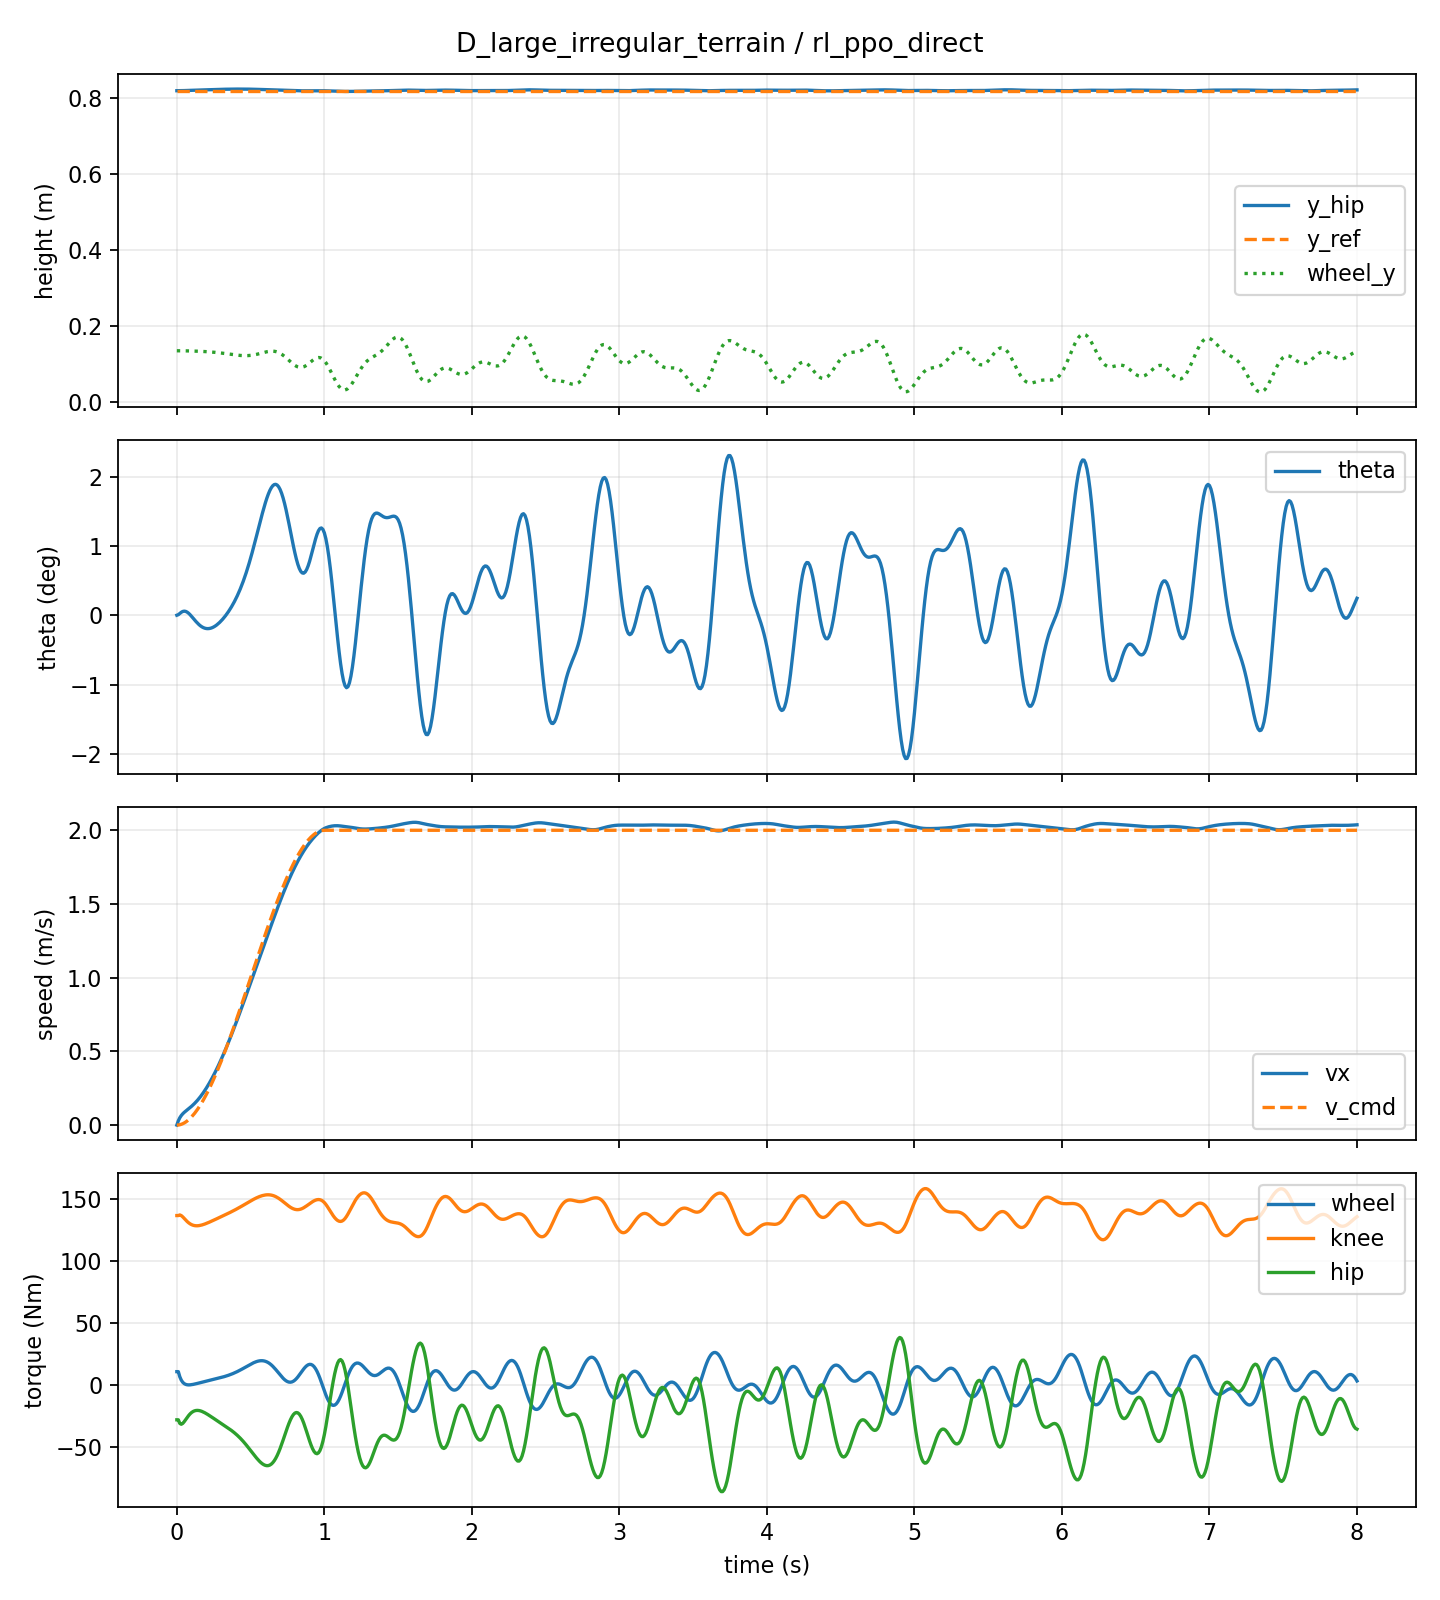
\includegraphics[width=\linewidth]{D_large_irregular_terrain__rl_ppo_direct.png}
\caption{直接 PPO}
\end{subfigure}
\caption{场景 D 的代表性单控制器曲线。}
\label{fig:scene-d}
\end{figure}

\subsection{场景 E：超规格组合压力}
\begin{table}[H]
\centering
\caption{场景 E 主要控制器结果}
\label{tab:scene-e}
\scriptsize\setlength{\tabcolsep}{3.0pt}
\begin{tabular}{lccccccc}
\toprule
控制器 & 状态 & $\mathrm{RMSE}_h$/m & $e_{h,\max}$/m & $\mathrm{RMSE}_\theta$ & $\theta_{\max}$ & $\mathrm{RMSE}_v$/m/s & 饱和比 \\
\midrule
LQR & \good & 0.02780 & 0.04651 & $0.4906^\circ$ & $0.6991^\circ$ & 0.5833 & 0 \\
WBC/QP & \good & \textbf{0.00019} & \textbf{0.00054} & \textbf{$0.0117^\circ$} & \textbf{$0.0207^\circ$} & 0.1996 & 0.0162 \\
PD 残差 PPO & \good & 0.00683 & 0.01267 & $2.6151^\circ$ & $2.7948^\circ$ & 0.3187 & 0.0017 \\
直接 PPO & \good & 0.00518 & 0.00814 & $1.3464^\circ$ & $2.8508^\circ$ & \textbf{0.0352} & 0.0083 \\
\bottomrule
\end{tabular}
\end{table}

\begin{figure}[H]
\centering

\includegraphics[width=\comparisonfigwidth]{E_combined_stress__controller_comparison.png}
\caption{场景 E 的五控制器叠加曲线。该场景峰值外力为 \SI{160}{N}，超出题目上限。}
\label{fig:scene-e-comparison}
\end{figure}

图~\ref{fig:scene-e-comparison} 给出组合压力场景下的五控制器叠加响应。该场景同时包含不规则地形、持续外力和
\SI{100}{N} 脉冲，外力峰值达到 \SI{160}{N}。图中的红色前馈残差曲线在速度通道持续偏离，其高度和姿态仍未超过
终止阈值；这说明“未终止”和“速度跟踪良好”在该场景中需要分开判断。图~\ref{fig:scene-e} 单独给出 WBC/QP 与
直接 PPO，便于观察两种代表性控制器在平台通道和速度通道上的差异。

表~\ref{tab:scene-e} 中，WBC/QP 的高度 RMSE 为 \SI{0.00019}{m}，姿态 RMSE 为
\SI{0.0117}{\degree}，速度 RMSE 为 \SI{0.1996}{m/s}，饱和比例为 $1.62\%$。直接 PPO 的速度 RMSE 为
\SI{0.0352}{m/s}，但其姿态 RMSE 为 \SI{1.3464}{\degree}，最大姿态角为 \SI{2.8508}{\degree}。LQR 的速度
RMSE 为 \SI{0.5833}{m/s}，PD 残差 PPO 为 \SI{0.3187}{m/s}。该场景超出题目外力上限，因此它在本文中用于观察
组合扰动下的响应形态，而不作为题目范围内的性能边界。

\begin{figure}[H]
\centering
\begin{subfigure}[t]{0.48\linewidth}
\centering
\includegraphics[width=\linewidth]{E_combined_stress__wbc_qp.png}
\caption{WBC/QP}
\end{subfigure}\hfill
\begin{subfigure}[t]{0.48\linewidth}
\centering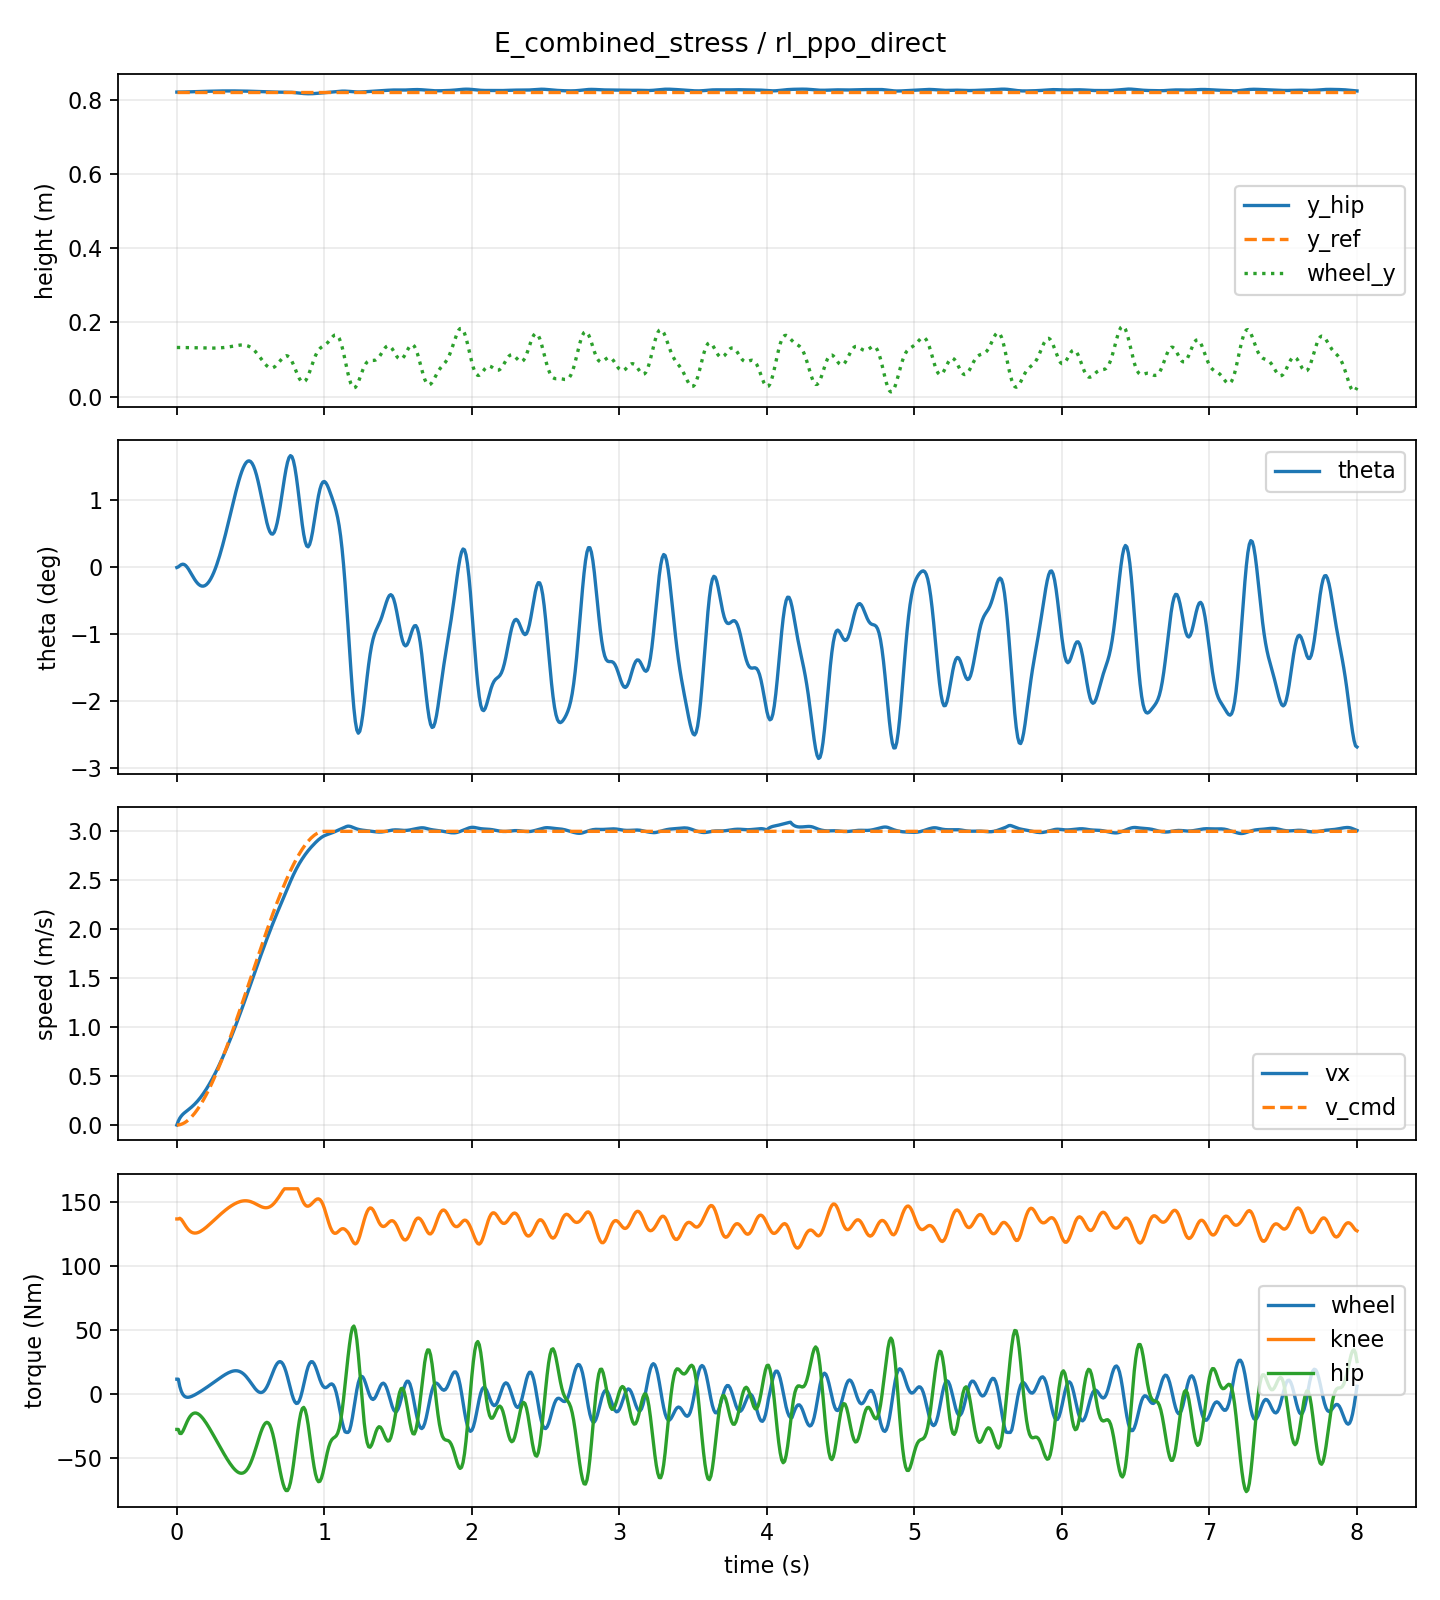
\includegraphics[width=\linewidth]{E_combined_stress__rl_ppo_direct.png}
\caption{直接 PPO}
\end{subfigure}
\caption{场景 E 的代表性单控制器曲线。}
\label{fig:scene-e}
\end{figure}

\begin{figure}[H]
\centering

\includegraphics[width=0.86\linewidth]{E_combined_stress__wbc_qp__diagnostics.png}
\caption{场景 E 的 WBC/QP 诊断图：接触力与摩擦边界、实际与预测腿长、残差与松弛量、摩擦利用率和求解状态。}
\label{fig:scene-e-diagnostics}
\end{figure}

图~\ref{fig:scene-e-diagnostics} 为场景 E 的 WBC/QP 诊断图，分别给出接触力与摩擦边界、实际腿长与预测腿长、
约束残差/松弛量、摩擦利用率和求解状态。对应的诊断数据中，最大摩擦利用率为 0.7507，QP 与 OSQP 状态均为
$100\%$ 成功，最大等式残差约 $1.14\times10^{-13}$，不等式违反量为零。平均 OSQP 求解耗时约
\SI{0.078}{ms}，最大约 \SI{1.31}{ms}。这些数值对应当前电脑、当前轨迹和当前降阶模型下的求解记录。

\subsection{场景 F：\SI{5}{m/s} 高速平地}
\begin{table}[H]
\centering
\caption{场景 F 主要控制器结果}
\label{tab:scene-f}
\scriptsize\setlength{\tabcolsep}{3.0pt}
\begin{tabular}{lccccccc}
\toprule
控制器 & 状态 & $\mathrm{RMSE}_h$/m & $e_{h,\max}$/m & $\mathrm{RMSE}_\theta$ & $\theta_{\max}$ & $\mathrm{RMSE}_v$/m/s & 饱和比 \\
\midrule
LQR & \good & 0.03179 & 0.11163 & $0.3699^\circ$ & $1.1325^\circ$ & 0.6686 & 0 \\
WBC/QP & \good & \textbf{0.00206} & \textbf{0.00723} & \textbf{$0.0394^\circ$} & \textbf{$0.1394^\circ$} & 0.7114 & 0.0633 \\
PD 残差 PPO & \good & 0.01743 & 0.06957 & $3.0037^\circ$ & $4.0707^\circ$ & 0.5200 & 0.0466 \\
直接 PPO & \good & 0.02296 & 0.08438 & $2.8114^\circ$ & $3.6182^\circ$ & \textbf{0.2942} & 0.0637 \\
\bottomrule
\end{tabular}
\end{table}

\begin{figure}[H]
\centering

\includegraphics[width=\comparisonfigwidth]{F_high_speed_flat__controller_comparison.png}
\caption{场景 F 的五控制器叠加曲线。速度 RMSE 包含从初始速度到 \SI{5}{m/s} 的完整启动过程。}
\label{fig:scene-f-comparison}
\end{figure}

图~\ref{fig:scene-f-comparison} 给出 \SI{5}{m/s} 高速平地场景的响应。速度子图包含从静止到目标速度的启动段，
因此全时域速度 RMSE 同时记录加速过程和接近稳态后的偏差。高度误差和力矩范数的峰值主要集中在启动初期，
该阶段也是不同控制器差异最明显的位置。

表~\ref{tab:scene-f} 中，直接 PPO 的速度 RMSE 为 \SI{0.2942}{m/s}，低于 WBC/QP 的
\SI{0.7114}{m/s}、LQR 的 \SI{0.6686}{m/s} 和 PD 残差 PPO 的 \SI{0.5200}{m/s}。WBC/QP 的高度 RMSE 为
\SI{0.00206}{m}，姿态 RMSE 为 \SI{0.0394}{\degree}，在平台通道上保持较小误差；其饱和比例为 $6.33\%$。
直接 PPO 的高度 RMSE 为 \SI{0.02296}{m}，姿态 RMSE 为 \SI{2.8114}{\degree}，饱和比例为 $6.37\%$。
LQR 的最大高度误差达到 \SI{0.11163}{m}，对应图中启动阶段的明显下沉。高速场景中，速度响应和平台姿态之间的
分配差异比中低速场景更突出。

\subsection{场景 G：题目边界组合}
\begin{table}[H]
\centering
\caption{场景 G 主要控制器结果}
\label{tab:scene-g}
\scriptsize\setlength{\tabcolsep}{3.0pt}
\begin{tabular}{lccccccc}
\toprule
控制器 & 状态 & $\mathrm{RMSE}_h$/m & $e_{h,\max}$/m & $\mathrm{RMSE}_\theta$ & $\theta_{\max}$ & $\mathrm{RMSE}_v$/m/s & 饱和比 \\
\midrule
LQR & \good & 0.04882 & 0.10259 & $0.8212^\circ$ & $0.9484^\circ$ & 1.0754 & 0.0079 \\
WBC/QP & \good & \textbf{0.00043} & \textbf{0.00189} & \textbf{$0.0141^\circ$} & \textbf{$0.0332^\circ$} & 0.3882 & 0.0270 \\
PD 残差 PPO & \good & 0.01070 & 0.04017 & $3.0175^\circ$ & $3.4555^\circ$ & 0.6364 & 0.0433 \\
直接 PPO & \good & 0.01536 & 0.02168 & $4.0563^\circ$ & $4.7711^\circ$ & \textbf{0.1587} & 0.0408 \\
\bottomrule
\end{tabular}
\end{table}

\begin{figure}[H]
\centering

\includegraphics[width=\comparisonfigwidth]{G_requirement_boundary__controller_comparison.png}
\caption{场景 G 的五控制器叠加曲线。该场景同时达到题目规定的速度和外力上限。}
\label{fig:scene-g-comparison}
\end{figure}

图~\ref{fig:scene-g-comparison} 对应题目边界组合场景，速度为 \SI{5}{m/s}，水平外力为 \SI{100}{N}，
地形为规则正弦起伏。该图同时显示高速启动、持续推力和地形周期扰动对四个通道的影响。图~\ref{fig:scene-g}
单独列出 WBC/QP 与直接 PPO：前者的高度和姿态曲线接近零线，后者的速度曲线更接近指令速度，但俯仰角波动更大。

表~\ref{tab:scene-g} 中，WBC/QP 的高度 RMSE 为 \SI{0.00043}{m}，姿态 RMSE 为
\SI{0.0141}{\degree}，速度 RMSE 为 \SI{0.3882}{m/s}，饱和比例为 $2.70\%$。直接 PPO 的速度 RMSE 为
\SI{0.1587}{m/s}，在表中最低；其姿态 RMSE 为 \SI{4.0563}{\degree}，最大姿态角为
\SI{4.7711}{\degree}。LQR 的速度 RMSE 为 \SI{1.0754}{m/s}，高度 RMSE 为 \SI{0.04882}{m}；
PD 残差 PPO 的速度 RMSE 为 \SI{0.6364}{m/s}，姿态 RMSE 为 \SI{3.0175}{\degree}。在最高速度、最大外力和
不平地形同时出现时，表格和曲线都显示出两类结果：WBC/QP 保持平台高度和姿态，直接 PPO 保持较低速度误差。

\begin{figure}[H]
\centering
\begin{subfigure}[t]{0.48\linewidth}
\centering
\includegraphics[width=\linewidth]{G_requirement_boundary__wbc_qp.png}
\caption{WBC/QP：平台稳定优先}
\end{subfigure}\hfill
\begin{subfigure}[t]{0.48\linewidth}
\centering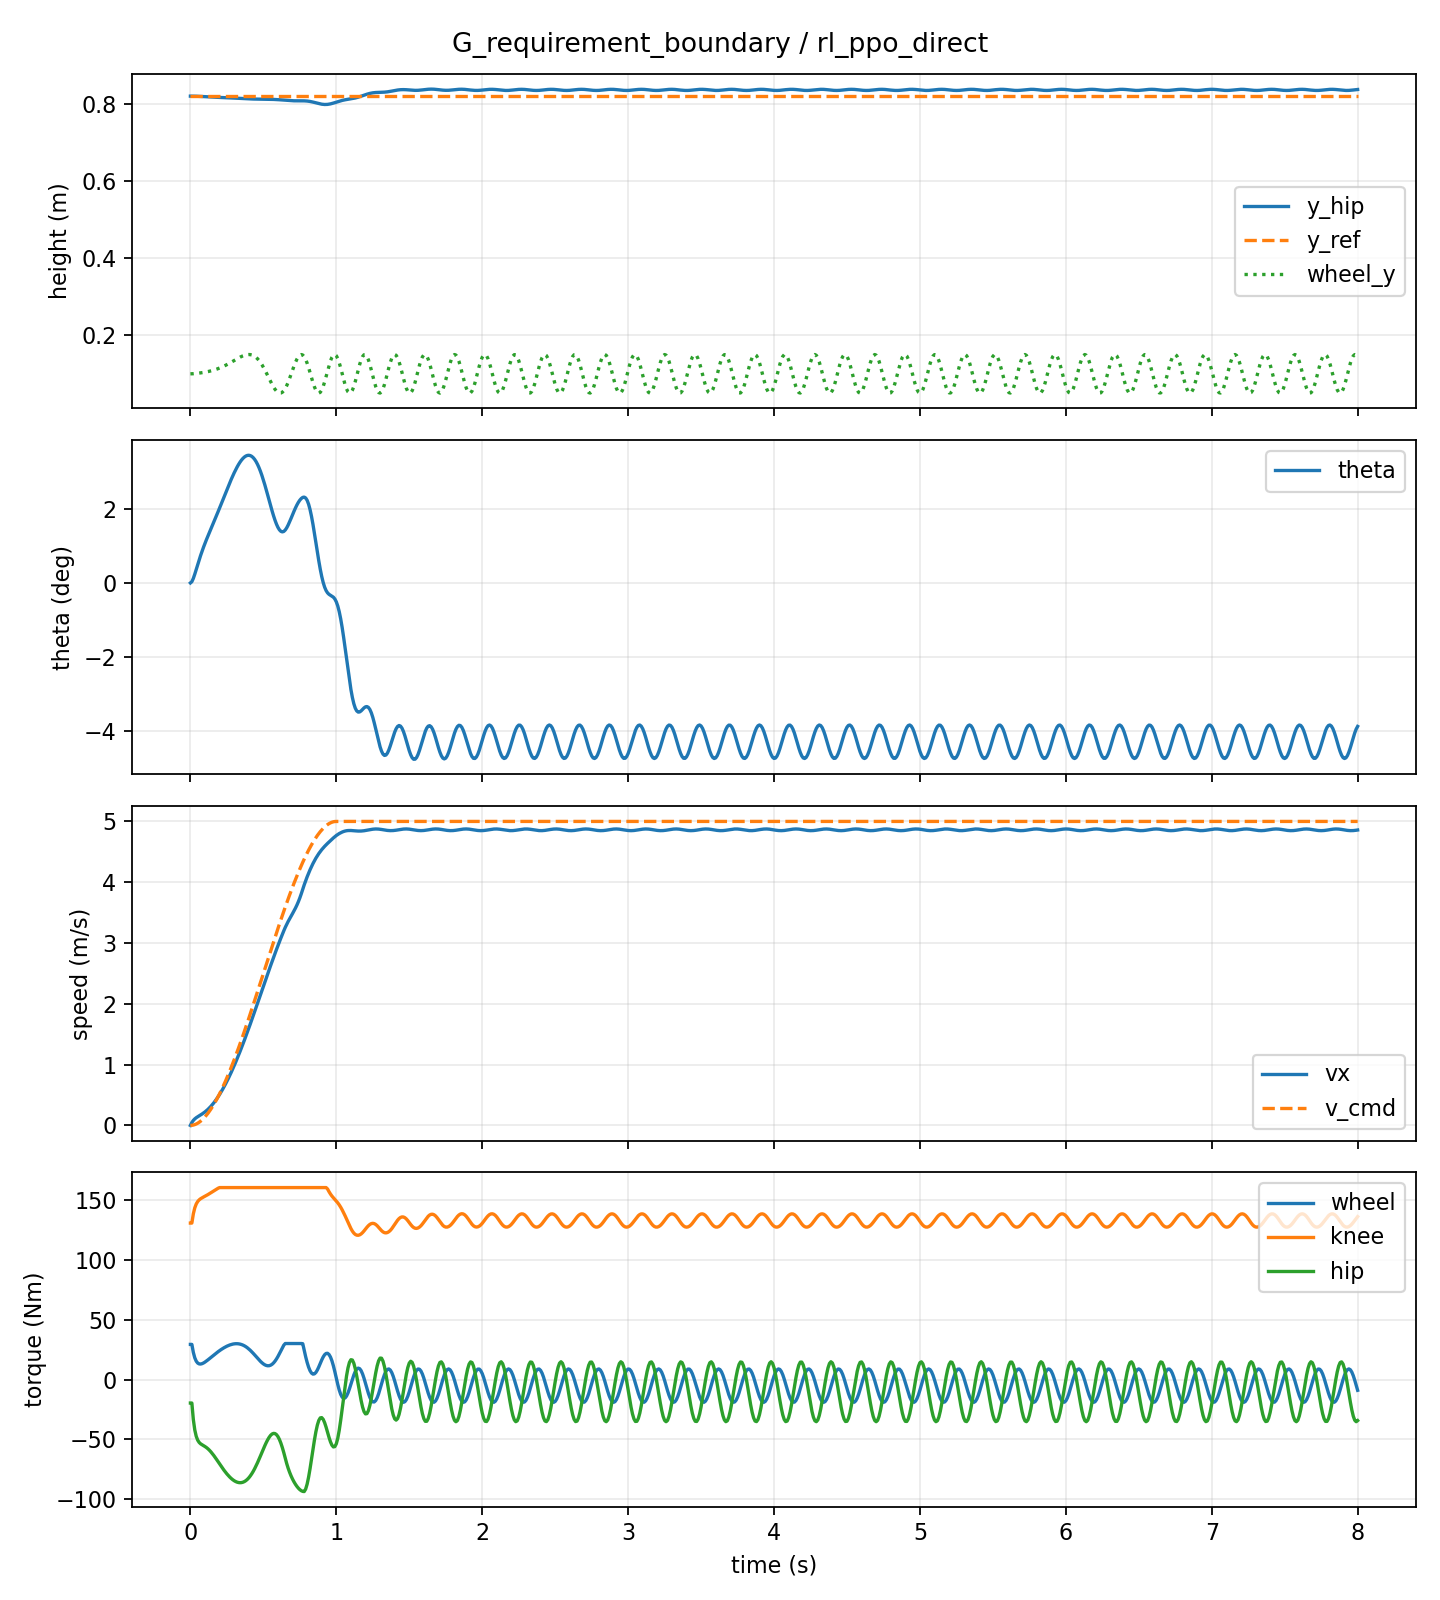
\includegraphics[width=\linewidth]{G_requirement_boundary__rl_ppo_direct.png}
\caption{直接 PPO：速度优先、姿态波动较大}
\end{subfigure}
\caption{场景 G 的代表性单控制器曲线。}
\label{fig:scene-g}
\end{figure}

\section{控制器比较与实现改进}

\subsection{LQR}
LQR 适合作为可解释、低计算量的基线。当前实现的主要不足不是算法本身，而是设计点和增广状态不足：
无外力估计、无积分、无地形调度，且线性化含不可微裁剪。可依次改进为：去掉绝对位置模态；加入速度积分构成
LQI；使用扰动观测器；按速度和坡度进行增益调度；最后再比较带输入约束的 MPC。

\subsection{降阶 WBC/QP}
WBC/QP 能直接表达任务权重、摩擦和执行器约束，适合作为当前平台稳定任务的主控制器候选。进一步改进应优先验证：
\begin{itemize}
  \item 对质量、惯量、摩擦、地形高度和坡度误差做参数扫描；
  \item 把 $F_n\ge0.35mg$ 的经验下界改为可解释的接触安全裕度，并做灵敏度分析；
  \item 将单步预瞄扩展为多步 MPC，避免高曲率地形下的局部近似误差；
  \item 复用 OSQP 工作区并统计完整控制周期，而非只统计求解器调用；
  \item 在高保真多刚体模型中验证主动支撑力映射和俯仰耦合系数。
\end{itemize}

\subsection{残差 PPO 与直接 PPO}
PD 残差 PPO 训练容易，但性能上限受基础反馈与残差幅值限制；前馈残差消融说明，去掉基础反馈后，当前训练预算
不足以让策略可靠承担全部稳定任务。直接 PPO 的速度误差最低，但姿态误差和可解释安全约束较弱。部署前需要
多随机种子训练、域随机化、观测噪声与时延训练、动作变化率限制，并在策略输出后增加 QP 安全过滤器或备用控制器。

\subsection{推荐方案}
对题目中“速度跟踪、躯干竖直、地形扰动和水平外力”同时存在的任务，本文推荐以降阶 WBC/QP 为主控制器，
理由是其任务优先级与约束可显式解释，并在边界场景 G 中给出最小高度与姿态误差。直接 PPO 可作为速度性能上限
和学习补偿模块；在当前证据下，直接 PPO 尚未作为安全关键主控制器使用。LQR 保留为基线和故障回退方案。

\section{复现方式与代码核验清单}

\subsection{依赖安装}
项目依赖由 \code{requirements.txt} 管理。在项目根目录执行：
\begin{lstlisting}[style=cmd]
python -m pip install -r requirements.txt
\end{lstlisting}

\subsection{建议的统一评估命令}
\begin{lstlisting}[style=cmd]
python -B scripts/run_compare.py \
  --controllers lqr wbc_qp rl_ppo rl_ppo_feedforward rl_ppo_direct \
  --residual-model-path outputs/models/ppo_wheel_leg_residual_random \
  --feedforward-model-path outputs/models/ppo_wheel_leg_feedforward_residual_random \
  --direct-model-path outputs/models/ppo_wheel_leg_direct \
  --out-dir outputs/compare_five_full_wbc
\end{lstlisting}

\subsection{训练与回归测试入口}
PPO 训练入口见下方命令；当前报告使用的检查点集中放在 \path{outputs/models/}。
典型训练命令如下：
\begin{lstlisting}[style=cmd]
python -B scripts/train_rl.py --action-mode residual \
  --scenario-set random_full --timesteps 300000 --n-envs 4 \
  --save-path outputs/models/ppo_wheel_leg_residual_random

python -B scripts/train_rl.py --action-mode feedforward_residual \
  --scenario-set random_full --timesteps 300000 --n-envs 4 \
  --save-path outputs/models/ppo_wheel_leg_feedforward_residual_random

python -B scripts/train_rl.py --action-mode direct \
  --scenario-set random_full --timesteps 1500000 --n-envs 8 \
  --load-path outputs/models/ppo_wheel_leg_direct_cont \
  --save-path outputs/models/ppo_wheel_leg_direct

python -B -m unittest discover -s tests -v
\end{lstlisting}




\subsection{主要源码映射}
\begin{table}[H]
\centering
\caption{报告内容与源码文件对应关系}
\label{tab:codemap}
\small
\begin{tabularx}{\linewidth}{p{5.2cm}Y}
\toprule
文件 & 作用 \\
\midrule
\path{src/config/params.py} & 机器人参数、仿真参数和安全阈值 \\
\path{src/config/scenarios.py} & 八个固定测试场景、速度平滑和外力函数 \\
\path{src/config/random_scenarios.py} & PPO 随机训练场景采样器 \\
\path{src/model/terrain.py} & 平地、正弦、多频和噪声地形 \\
\path{src/model/kinematics.py} & 轮心高度、腿长、逆运动学和 RL 观测量 \\
\path{src/model/dynamics.py} & 前向动力学、RK4 积分、失败检测和 WBC 仿射模型 \\
\path{src/controllers/base.py} & 控制器接口、平衡力矩、残差动作和直接动作映射 \\
\path{src/controllers/lqr.py} & 数值线性化、CARE 求解和 LQR 控制律 \\
\path{src/controllers/wbc_qp.py} & 降阶 WBC/QP 的目标、约束、OSQP 求解与诊断量 \\
\path{src/controllers/rl_policy.py} & PPO 模型加载、残差/前馈/直接策略适配器 \\
\path{src/rl/env.py} & Gymnasium 环境、奖励函数和训练终止逻辑 \\
\path{src/simulation/runner.py} & 统一仿真循环、盲扰动开关和日志采样 \\
\path{src/evaluation/metrics.py} & 指标计算和 CSV 输出 \\
\path{src/evaluation/plots.py} & 单控制器图、叠加对比图和 WBC 诊断图 \\
\path{tests/test_core_logic.py} & 动力学、场景、日志和题目边界的回归测试 \\
\bottomrule
\end{tabularx}
\end{table}


\section{结论}
本文在统一二维降阶平台上比较了 LQR、降阶 WBC/QP 和三种 PPO 结构。结果支持以下结论：
\begin{enumerate}
  \item 五种实现均未触发当前安全终止阈值，但前馈残差 PPO 的严重速度偏差说明安全成功率不能替代任务性能指标。
  \item WBC/QP 在高度和姿态指标上最优，尤其适合平台稳定优先的任务；其极小误差受到共享精确模型和地形预瞄条件的显著影响。
  \item 直接 PPO 的速度 RMSE 最低，但在高速组合场景中姿态波动明显，尚需安全过滤和更系统的泛化验证。
  \item LQR 作为基线稳定可靠，但缺少积分、扰动估计和地形适应时，持续外力与高速组合工况下速度误差较大。
  \item 当前实验是确定性课程仿真比较，不是实机稳定性证明。下一步应加入多随机种子、参数失配、传感器噪声、时延、接触切换和高保真多刚体模型。
\end{enumerate}

从题目目标出发，推荐采用 WBC/QP 作为主要控制器，并把 LQR 用作简洁基线，把 PPO 用作速度补偿或策略对照。
该结论只对当前模型、权重、限幅和八个测试场景成立。

\clearpage
\addcontentsline{toc}{section}{参考文献}
\begin{thebibliography}{99}

\bibitem{Bjelonic2019KeepRollin}
M.~Bjelonic, R.~Grandia, P.~Fankhauser, O.~Harley, C.~D.~Bellicoso, and M.~Hutter.
\newblock Keep Rollin'--Whole-Body Motion Control and Planning for Wheeled Quadrupedal Robots.
\newblock \emph{IEEE Robotics and Automation Letters}, 4(2):2116--2123, 2019.

\bibitem{Kalman1960OptimalControl}
R.~E.~Kalman.
\newblock Contributions to the theory of optimal control.
\newblock \emph{Boletin de la Sociedad Matematica Mexicana}, 5:102--119, 1960.

\bibitem{AndersonMoore1990OptimalControl}
B.~D.~O.~Anderson and J.~B.~Moore.
\newblock \emph{Optimal Control: Linear Quadratic Methods}.
\newblock Prentice Hall, 1990.

\bibitem{Khatib1987OperationalSpace}
O.~Khatib.
\newblock A unified approach for motion and force control of robot manipulators: The operational space formulation.
\newblock \emph{IEEE Journal on Robotics and Automation}, RA-3(1):43--53, 1987.

\bibitem{Stellato2020OSQP}
B.~Stellato, G.~Banjac, P.~Goulart, A.~Bemporad, and S.~Boyd.
\newblock OSQP: an operator splitting solver for quadratic programs.
\newblock \emph{Mathematical Programming Computation}, 12:637--672, 2020.
\newblock \url{https://web.stanford.edu/~boyd/papers/osqp.html}

\bibitem{Schulman2017PPO}
J.~Schulman, F.~Wolski, P.~Dhariwal, A.~Radford, and O.~Klimov.
\newblock Proximal Policy Optimization Algorithms.
\newblock arXiv:1707.06347, 2017.
\newblock \url{https://arxiv.org/abs/1707.06347}

\bibitem{Towers2024Gymnasium}
M.~Towers et al.
\newblock Gymnasium: A Standard Interface for Reinforcement Learning Environments.
\newblock arXiv:2407.17032, 2024.
\newblock \url{https://arxiv.org/abs/2407.17032}

\bibitem{Raffin2021SB3}
A.~Raffin, A.~Hill, A.~Gleave, A.~Kanervisto, M.~Ernestus, and N.~Dormann.
\newblock Stable-Baselines3: Reliable Reinforcement Learning Implementations.
\newblock \emph{Journal of Machine Learning Research}, 22(268):1--8, 2021.
\newblock \url{https://jmlr.org/papers/v22/20-1364.html}

\end{thebibliography}

\end{document}
